% Template for ICIP-2015 paper; to be used with:
%          spconf.sty  - ICASSP/ICIP LaTeX style file, and
%          IEEEbib.bst - IEEE bibliography style file.
% --------------------------------------------------------------------------
\documentclass{article}
\usepackage{spconf,amsmath,graphicx}
\usepackage[utf8]{inputenc} % Suporte para acentuação sem necessidade dos comandos especiais.
\usepackage{amsmath,epsfig}
\usepackage[portuguese,algoruled,longend]{algorithm2e}
\usepackage{multirow}
\usepackage{MnSymbol}
\usepackage{wasysym}
\usepackage[table,xcdraw]{xcolor}
\usepackage[brazilian]{babel}
\usepackage{url}
\usepackage{float}
\usepackage{enumerate}
\usepackage[inline]{enumitem}
\usepackage{soul,framed} %,caption
\usepackage{matlab-prettifier}
\colorlet{shadecolor}{yellow}

% Template includegraphics
% \begin{figure}[H]
% 	\begin{center}
% 		\label{fig:11}
% 		\includegraphics[width=2.5in]{Figures/S02_Grafico_Ajustado.png}
% 		\caption{Gráficos da Situação 03 Ajustados}
% 	\end{center}
% \end{figure}  

% Example definitions.
% -------------------
\def\x{{\mathbf x}}
\def\L{{\cal L}}

% Title.
% ------
\title{Projeto 02 - Desenvolvimento de ferramentas computacionais para análise tempo-frequência}
%
% Single address.
% ---------------
\name{Davi de Alencar Mendes - 16/0026415}
\address{Engenharia Eletrônica, UnB-FGA, Brasília, Brasil}


\begin{document}

\maketitle

% \begin{abstract}

% \end{abstract}

% \begin{keywords}

% \end{keywords}

\section{Introdução}\label{sec:intro}
A utilização de ferramentas como espectrograma (baseados na Transformada de Fourier de Tempo Curto - \textit{STFT})  e escalograma (baseado em transformada Wavelet Discreta - \textit{DWT}) provê informações de interesse a respeito do comportamento dinâmico do sinal. Essas informações podem ser utilizada para extração de características. O presente trabalho aborda o desenvolvimento computacional dessas ferramentas no ambiente de programação MATLAB.

\section{Projeto}
\subsection{Espectrograma}
O espectrograma desenvolvido emprega a \textit{STFT} para analisar o comportamento em frequência em versões janeladas do sinal. O algoritmo desenvolvido permite ainda a utilização de janelas configuráveis e sobreposição de janelas bem como variar a quantidade de pontos utilizados para cálculo da FFT. O algoritmo desenvolvido é apresentado anexo ao trabalho.

\paragraph*{Sinal do tipo Chirp Linear}
Inicialmente, foi realizado um teste com um sinal do tipo Chirp que apresentação uma variação constante da frequência de acordo com $f(t) = 20 \times t$.
\begin{figure}[H]
	\begin{center}
		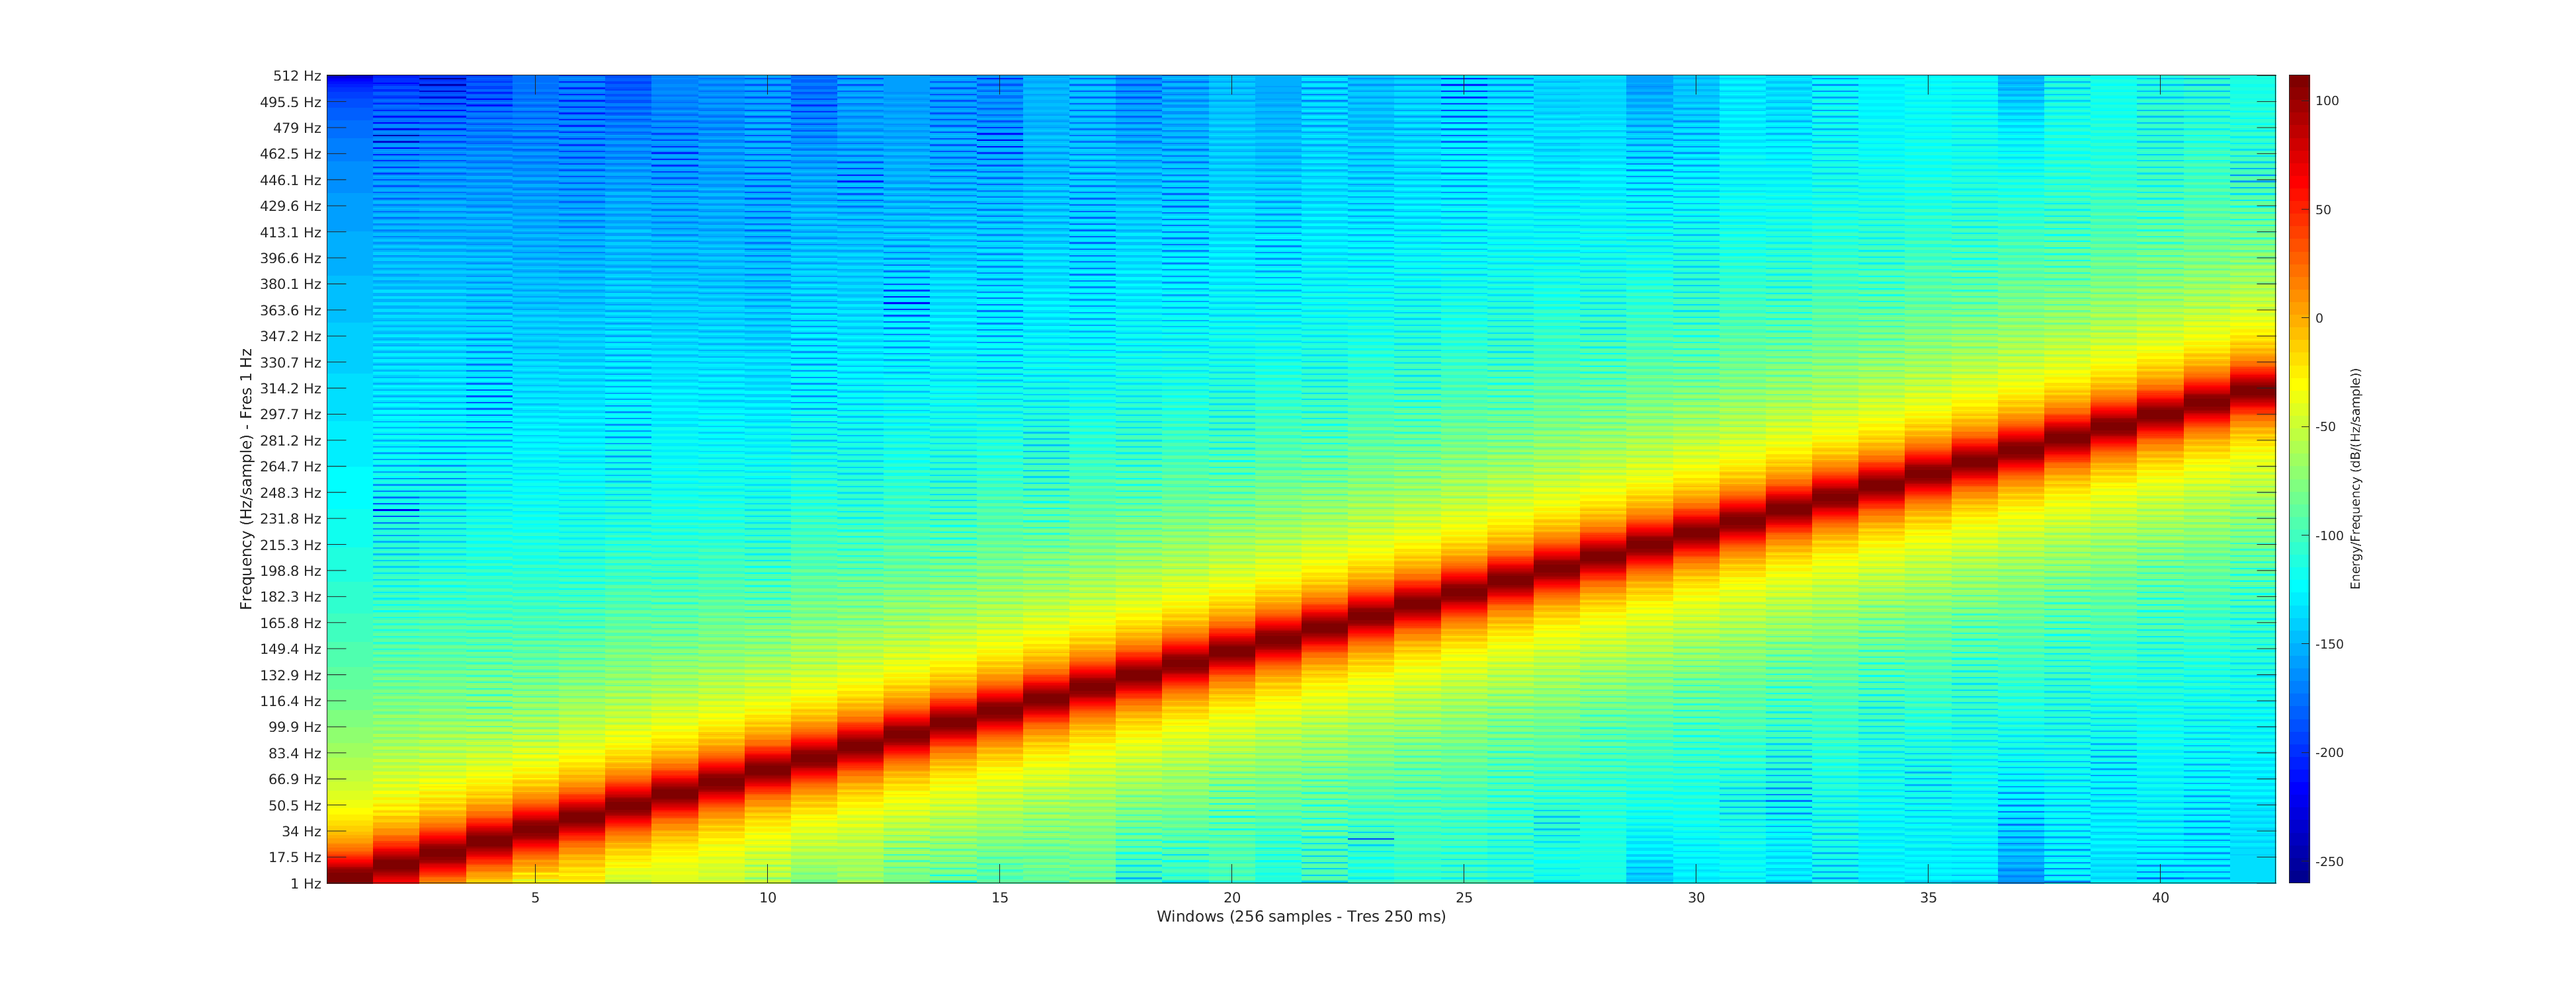
\includegraphics[width=3.5in]{Figures/linear_chirp_spectrogram.png}
		\caption{Espectrograma para sinal do tipo Chirp Linear}
		\label{fig:chirp}
	\end{center}
\end{figure}  

\paragraph*{Esteganografia - Gatos!}
Esteganografia é o estudo e uso de técnicas para ocultação de uma mensagem dentro de outra. Trata-se de uma forma de segurança por obscurantismo. Uma dessas abordagens consiste em esconder uma imagem em um segmento de aúdio de maneira que a imagem possa ser recuperada por meio visualização do espectrograma.

A música \textit{Look} produzida pelo artista Venetian Snares faz o uso da técnica citada para esconder imagens de gatos no espectrograma \cite{ref:cats}. A análise do conteúdo espectral da música contida em um arquivo de áudio MP3 revela os felinos escondidos!
\begin{figure}[H]
	\begin{center}
		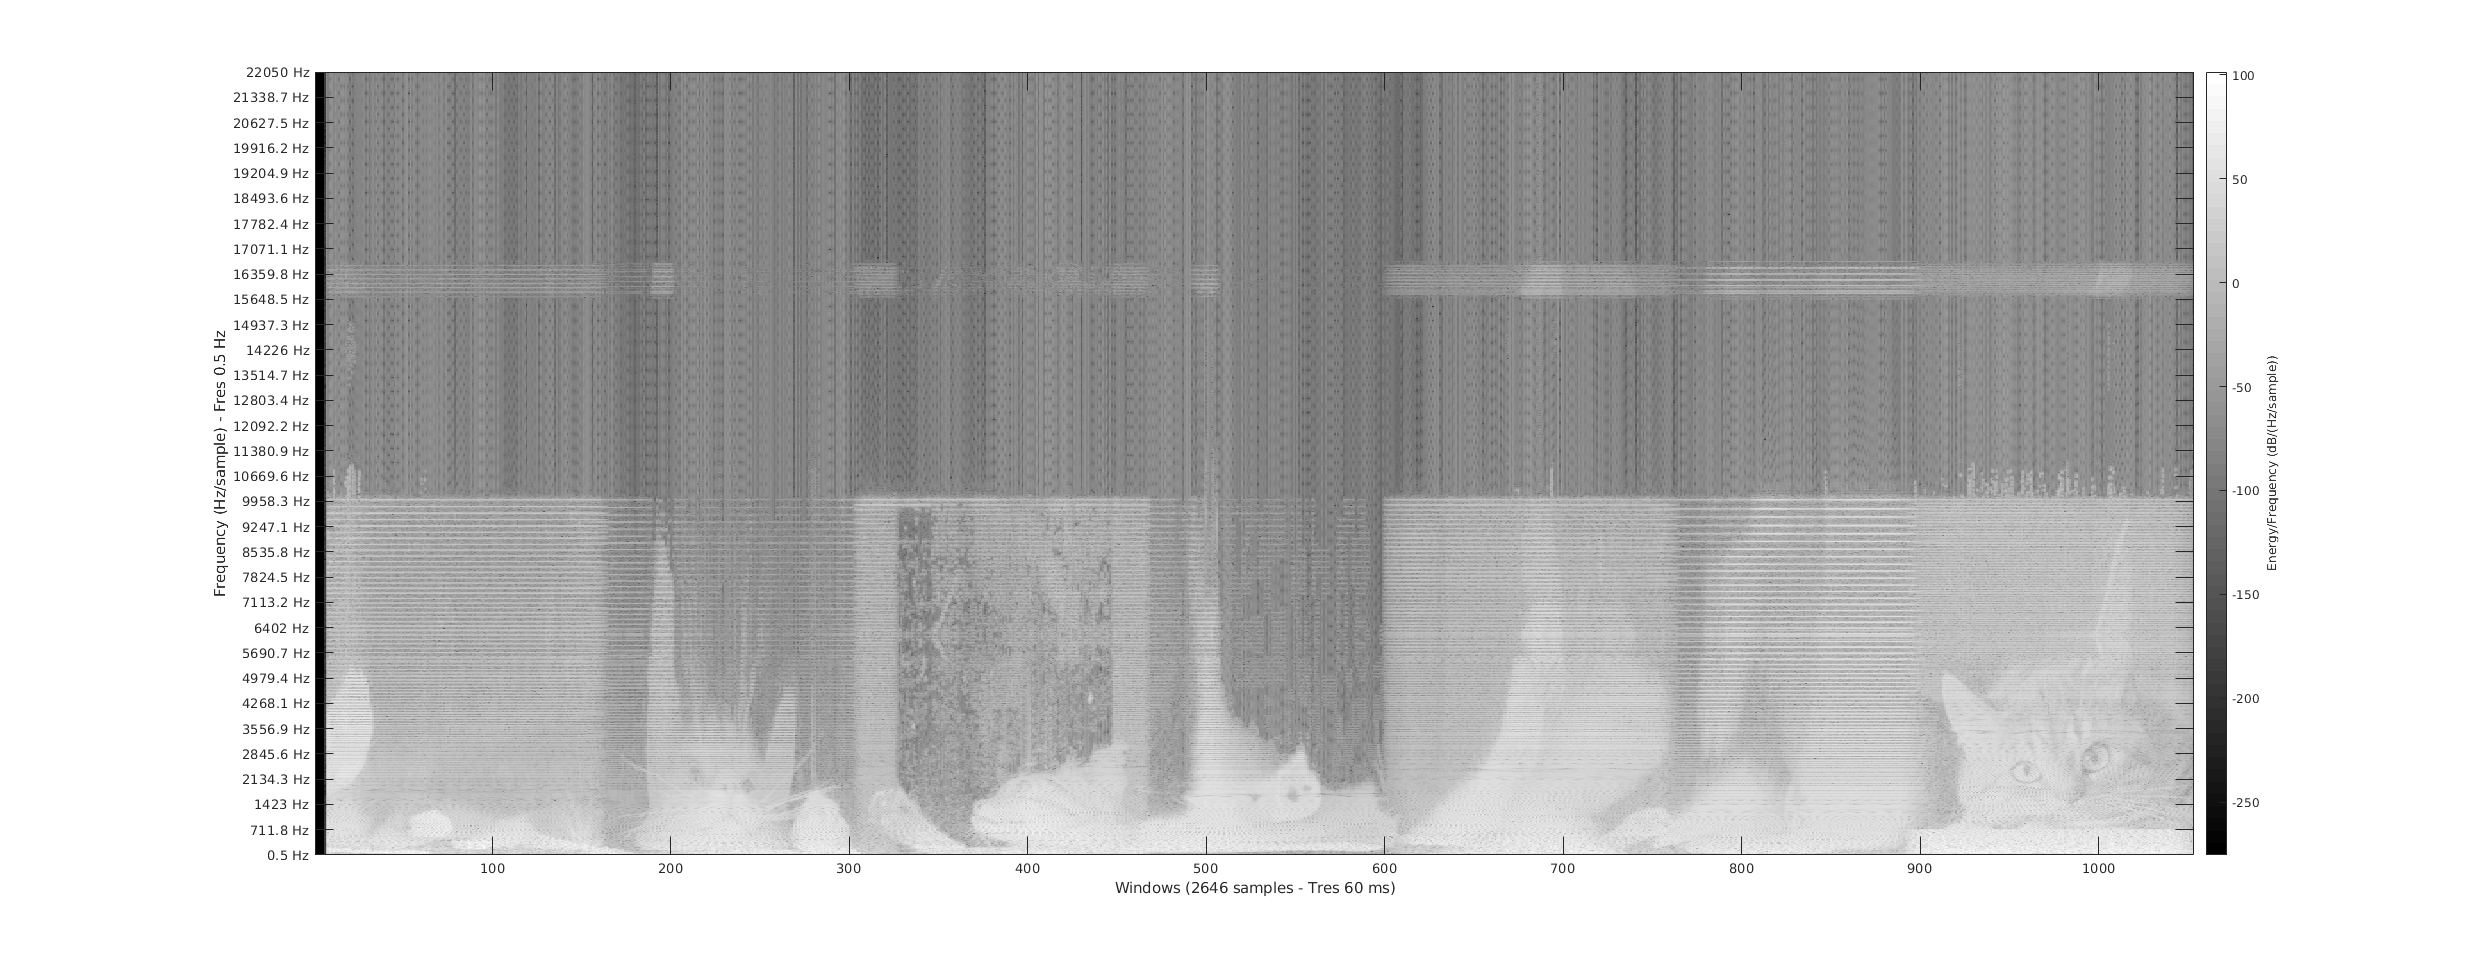
\includegraphics[width=3.5in]{Figures/cats.png}
		\caption{Espectrograma para Venetian Snares - \textit{Look}}
		\label{fig:cats}
	\end{center}
\end{figure}  

O procedimento para recuperação da imagem consistiu em isolar um canal do áudio em estéreo para análise via espectrograma. A taxa de amostragem do sinal foi de 44.1 kHz, típica para sinais de áudio codificados em MP3. Ademais, o \textit{bitrate} é de 95 kbps valor para o qual é obtida uma qualidade similar a de uma rádio FM \cite{ref:sayood}. Usando janelas de 60 ms com 50\% de sobreposição do tipo Hamming foi possível os resultados mostrados na figura ~\ref{fig:cats}.

Em especial, percebe-se que metade do espectrograma apresenta baixa concentração de energia. Possivelmente a codificação em MP3, que impõe perdas, levou a redução da largura de banda do sinal causando grandes perdas no conteúdo da imagem. Entretanto, ainda é possível observar os gatos presentes nas regiões de baixa frequência (vide figura ~\ref{fig:cats2}).

\begin{figure}[H]
	\begin{center}
		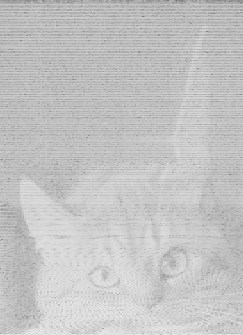
\includegraphics[width=2.5in]{Figures/crop_cats.png}
		\caption{Recorte do Espectrograma no qual observa-se um gato}
		\label{fig:cats2}
	\end{center}
\end{figure}  

\section{Escalograma}
Com a aplicação de técnicas multiresolução é possível obter representações tempo-frequência para as quais há uma melhor divisão do plano tempo-frequência conforme a figura ~\ref{fig:tf}.
\begin{figure}[H]
	\begin{center}
		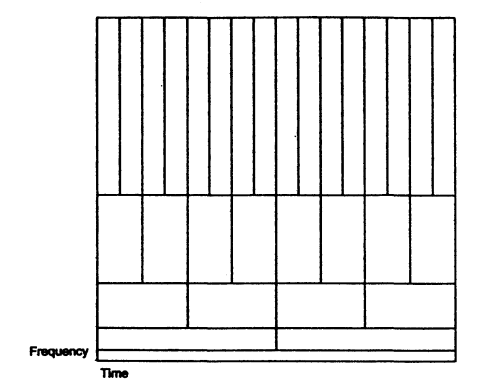
\includegraphics[width=2.5in]{Figures/tf_plane.png}
		\caption{Divisão Idealizada do plano Tempo-Frequência com wavelets - O tamanho da janela varia de maneira que em baixa frequências há melhor representação do tempo e em altas frequências há melhor resolução em frequência. Retirado de: \textit{The World According to Wavelets}}
		\label{fig:tf}
	\end{center}
\end{figure}

O escalograma desenvolvido emprega transformada discreta de Wavelets para compor uma visualização bastante similar ao espectrograma. A visualização permite observar quanto cada coeficiente é representativo em energia percentual para toda a escala mostrada. O número de escalas é determinado de acordo com o número de níveis da decomposição QMF utilizada. Como a decomposição QMF gera uma transformada com coeficientes de diferentes comprimentos foi empregada uma interpolação linear usando a técnica do vizinho mais próximo para que os níveis com menos coeficientes adequem-se ao grid presente na imagem de acordo com a divisão em termos da frequência de amostragem.

Para testar foi utilizado um sinal do tipo $x(t) = t^2\times-1^{fs \times t} + sen(10 \times t)$. Nota-se que há uma componente oscilatória de baixa frequência e uma componentes de alta frequência no sinal $x(t)$ mostrado na figura ~\ref{fig:x}.
\begin{figure}[h]
	\begin{center}
		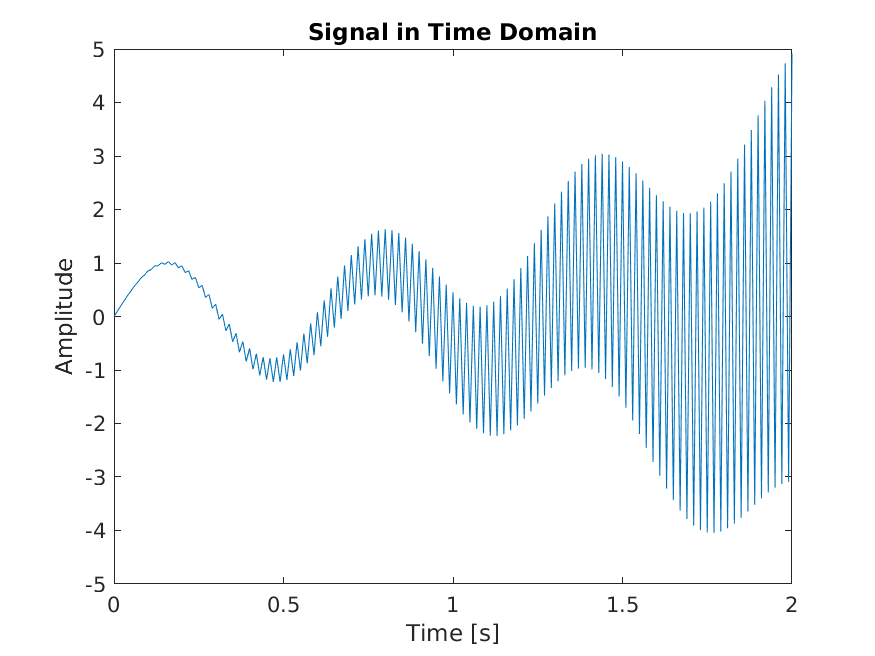
\includegraphics[width=2.5in]{Figures/scalogram_signal.png}
		\caption{sinal $x(t)$ representado no tempo}
		\label{fig:x}
	\end{center}
\end{figure}

Utilizando uma decomposição de 2 níveis com a Wavelet de Haar é possível obter o escalograma mostrado na figura ~\ref{fig:sc}. Na menor escala nota-se o comportamento de alta frequência apresentado no sinal em domínio temporal. Para as demais escalas, nota-se um comportamento oscilatório que é também característico do sinal.
\begin{figure}[h]
	\begin{center}
		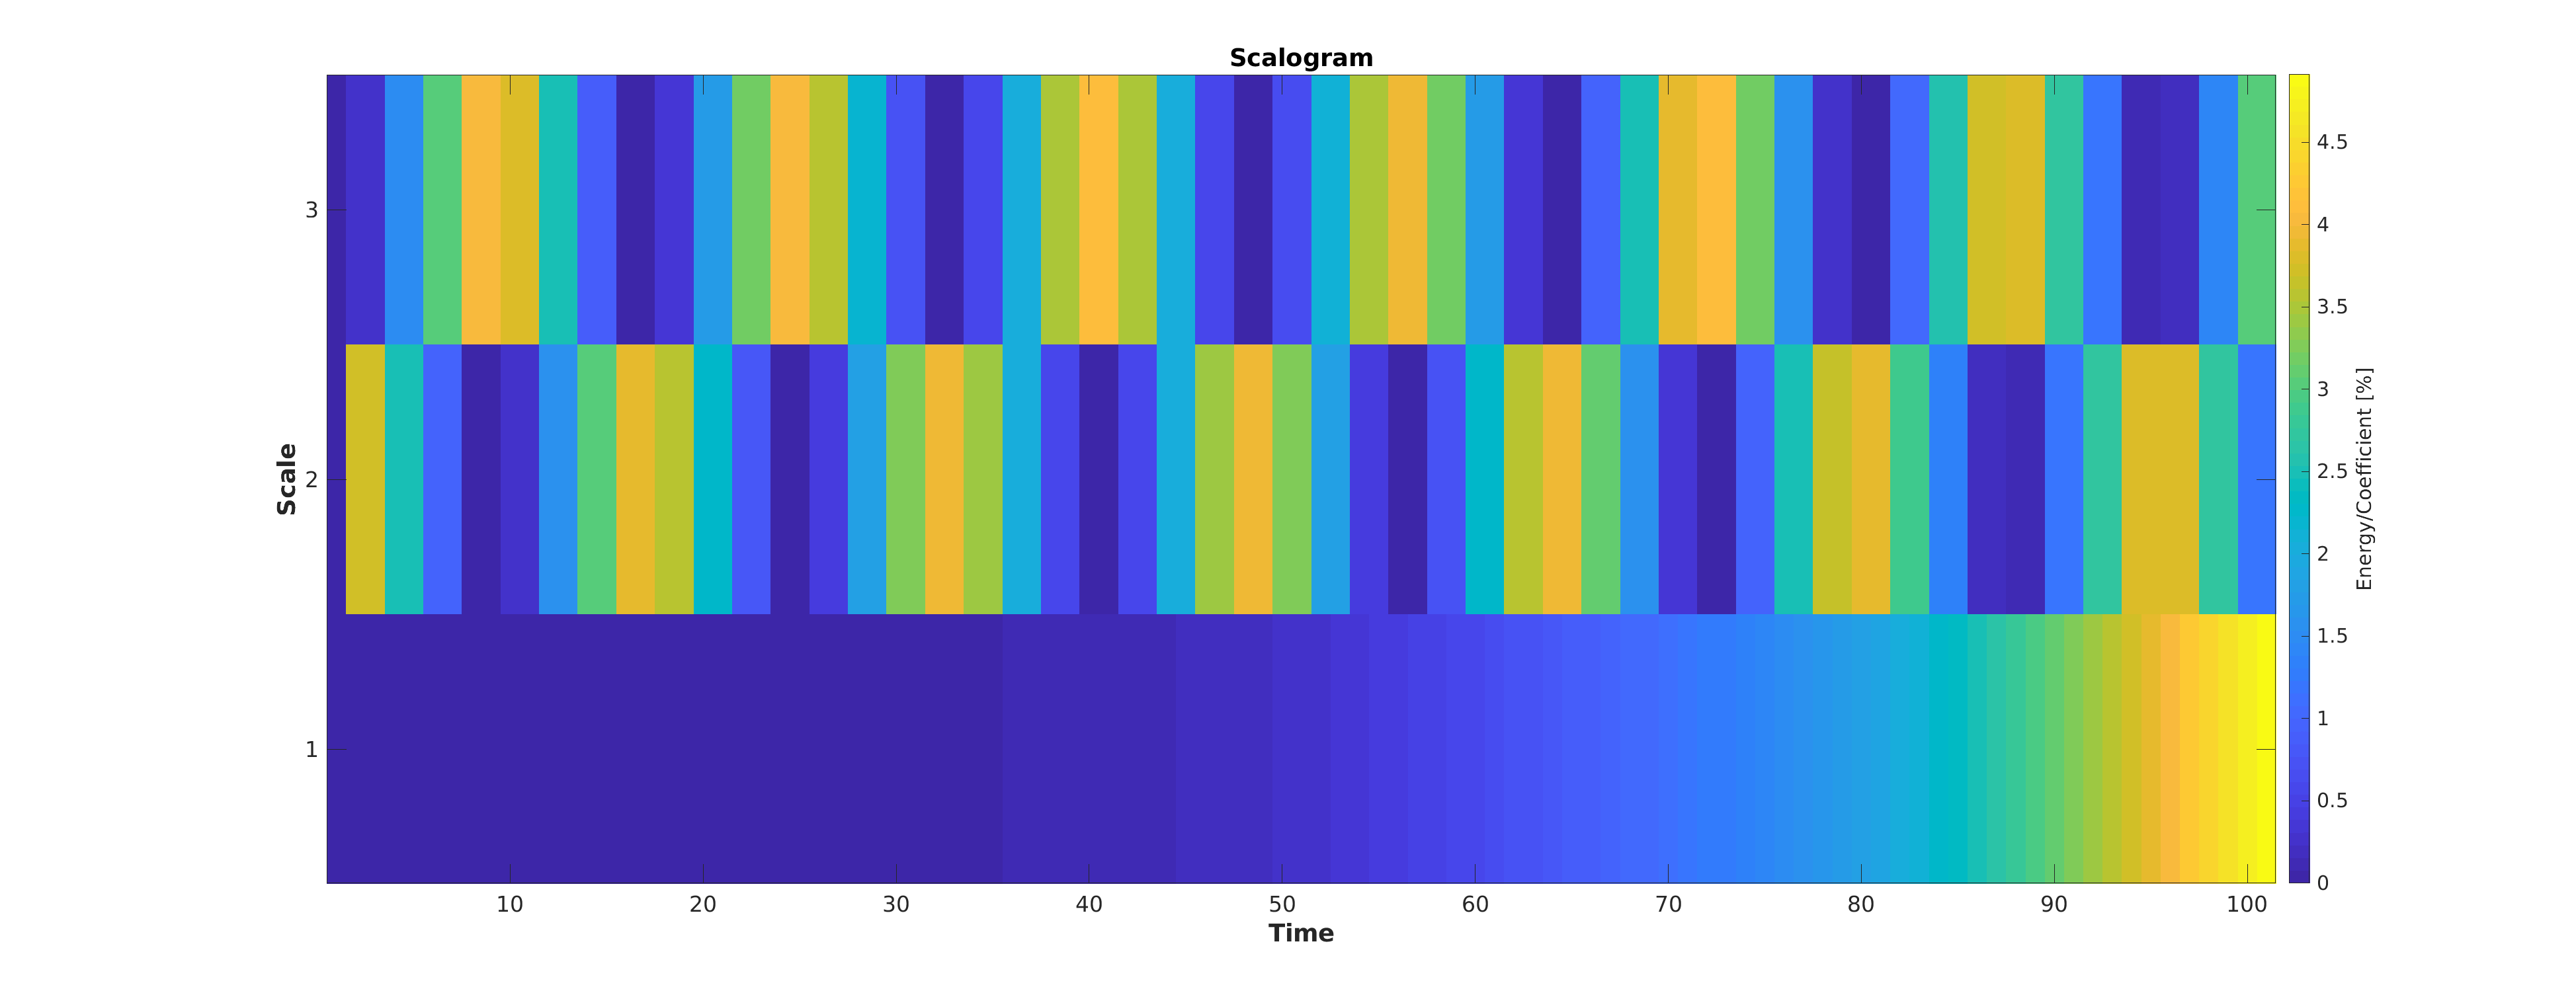
\includegraphics[width=3.5in]{Figures/scalogram.png}
		\caption{Escalograma para x(t)}
		\label{fig:sc}
	\end{center}
\end{figure}

\section{Extração de Características}
Por último, foi desenvolvido uma algoritmo para extração de características de um sinal. A extração de características é executada em uma janela de tempo do sinal, podendo haver sobreposição entre janelas. As características temporais escolhidas foram:
\begin{enumerate*}[label=(\roman*)]
	\item Valor Eficaz (RMS);
	\item Valor Médio Retificado (RMV);
	\item Desvio Padrão (STD).
\end{enumerate*}
As características espectrais escolhidas são aplicadas a cada uma das bandas definidas em frequência, podendo haver sobreposição entre bandas adjacentes. Sendo elas:
\begin{enumerate*}[label=(\roman*)]
	\item Energia;
	\item Frequência Média;
	\item Frequência Mediana;
	\item Frequência Modal.
\end{enumerate*}

Os testes para avaliar a coerência do extrator de características foram realizados com a comparação entre uma gravação do set A e outra do set E. É evidente que haverá uma grande separação das características já que tratam-se de pacientes saudáveis \textit{vs.} acometidos com epilepsia. Os resultados obtidos são mostrados nas figuras a seguir.

\begin{figure}[h]
	\begin{center}
		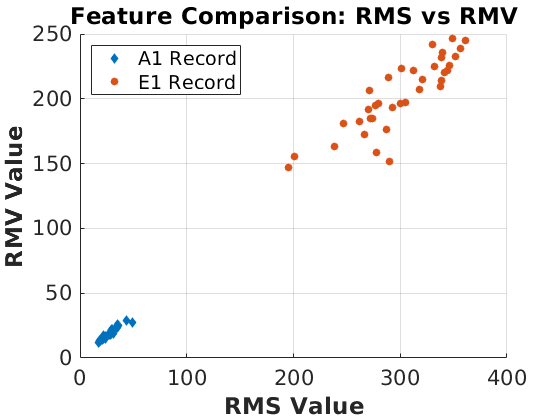
\includegraphics[width=3.5in]{Figures/rms_rmv.png}
		\caption{Comparação de características temporais}
		\label{fig:tf}
	\end{center}
\end{figure}

\begin{figure}[H]
	\begin{center}
		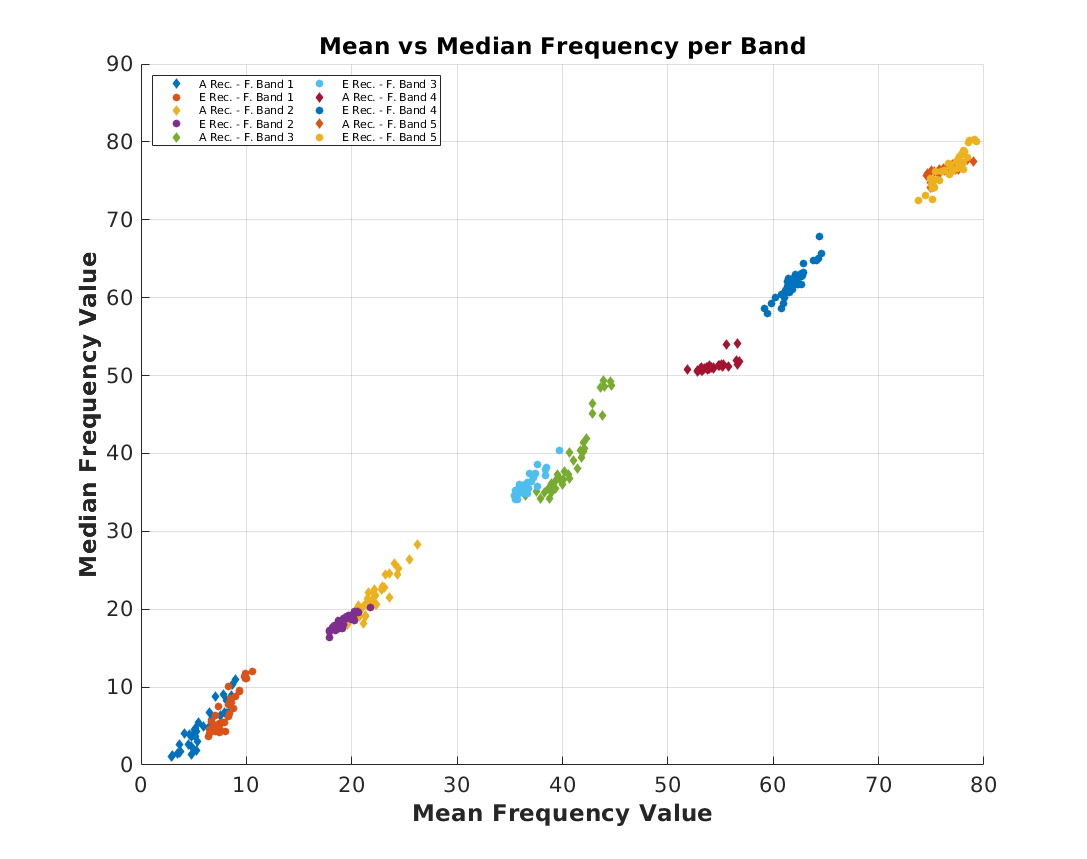
\includegraphics[width=3.5in]{Figures/mf_mf.png}
		\caption{Comparação de características espectrais}
		\label{fig:ff}
	\end{center}
\end{figure}

% -------------------------------------------------------------------------
\begin{thebibliography}{1}

\bibitem{ref:cats}
Bastwood Blog: The Aphex Face - \url{http://www.bastwood.com/?page_id=10}

\bibitem{ref:sayood}
Sayood, K. (2017). Introduction to Data Compression 5th Ed. (Chapter 17: Audio Coding) Morgan Kaufmann.


\end{thebibliography}

\onecolumn
\section*{Anexos}
\subsection*{Espectrograma - STFT}
\lstinputlisting[style=Matlab-editor]{../stftSpectrogram.m}
\subsection*{Espectrograma - Teste com Sinal Chirp \& Esteganografia}
\lstinputlisting[style=Matlab-editor]{../my_spectrogram.m}

\subsection*{Escalograma - DWT}
\lstinputlisting[style=Matlab-editor]{../dwtScalogram.m}
\subsection*{Escalograma - Rotina de Teste}
\lstinputlisting[style=Matlab-editor]{../my_scalogram.m}

\subsection*{Extração de Características}
\lstinputlisting[style=Matlab-editor]{../featureExtractor.m}
\subsection*{Extração de Características - Teste com sinais de EEG}
\lstinputlisting[style=Matlab-editor]{../demo_eeg_features.m}

\end{document}
